\documentclass[french]{msereport}

\usepackage{minted}

\newcommand{\openstack}{\brand{OpenStack}}
\newcommand{\openstackapi}{\brand{OpenStack API}}
\newcommand{\switchengines}{\brand{SWITCH Engines}}
\newcommand{\mongodb}{\brand{MongoDB}}

\title{Déploiement d'une application distribuée \\ sur \switchengines\ avec \openstack}
\module{CLOUD}{Cloud Computing}
\author{Jonathan Cornaz}

\begin{document}

	\section{Introduction}
		Ces exercices portaient sur le déploiement de machines chez \switchengines, dans le but de pouvoir concrètement manipuler des machines virtuelles chez un fournisseur de \eng{Cloud}.

		Pour cela, il était question de mettre en place trois serveurs qui dialoguerais entre eux :
		\begin{itemize}
			\item Une base de donnée \mongodb\ pour stocker des données.
			\item Un client \acs{REST} responsable d'aller chercher ces données sur des \eng{web-services} existants et mis à notre disposition pour les enregistrer dans la base de donnée.
			\item Un serveur \acs{REST} responsable de lire les données dans \mongodb\ pour les exposer sous forme de \eng{web-services}
		\end{itemize}

		Ces exercices ont été effectuées en utilisant le \eng{data-center} de \switchengines\ à Lausanne.

	\subtitledsection[Exercice 1]{Utiliser le portail de \switchengines\ pour déployer des machines}
		Pour réaliser le premier exercice, il a suffit de créer trois instances (\mongodb, \acs{REST} Serveur et \acs{REST} Client) sur \switchengines. Pour chacune des trois instances, une adresse \acs{IP} flottante a été attribué afin de permettre de directement s'y connecter via un \acs{SSH}.

		Une fois instanciées, les machines ont été installées et configurées selon la marche à suivre donnée. Les machines ont été sauvegardées (\eng{snapshot}) afin de pouvoir les instancier plus tard sans avoir à ré-effectuer l'installation et la configuration.

		Pour connecter les trois machines entre elles, l'adresse \acs{IP} locale a été utilisée. En effet, cela permet de n'utiliser qu'une seule adresse \acs{IP} flottante pour le serveur \acs{REST}. De plus cela est également intéressant d'un point du point de vue de la sécurité, car cela permet de ne pas avoir à exposer sur le web les deux autres machines.

		\begin{figure}[h]
			\label{instances}
			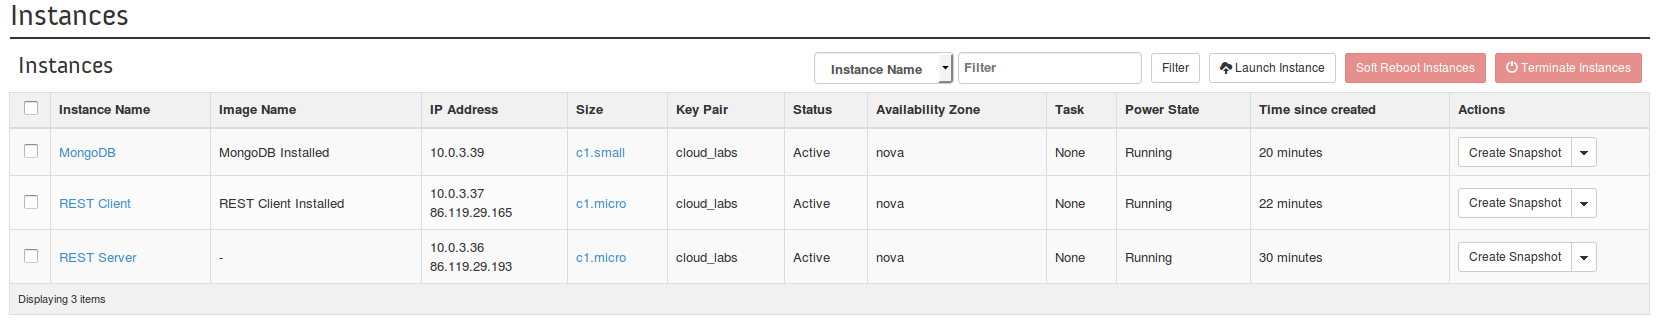
\includegraphics[width=\textwidth]{screen_instances.png}
			\caption{Instances démarrées sur \switchengines}
		\end{figure}

		\begin{figure}[h]
			\label{result}
			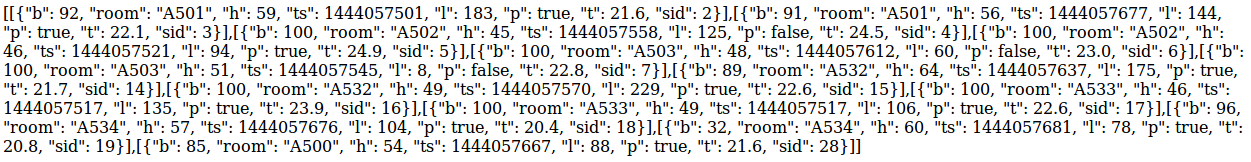
\includegraphics[width=\textwidth]{screen_sensors.png}
			\caption{Données des senseurs obtenues}
		\end{figure}

		Les données de la figure \ref{result} ont été obtenues le 5 octobre à 17h12 à l'\acs{URL} suivante : \url{http://86.119.29.193:18000/getLastSensorsValues/pi1}.

	\subtitledsection[Exercice 2]{Créer son réseau privé}
		Un réseau privé à été créé selon la marche à suivre. Une passerelle le relie au réseau publique et il dispose d'un routeur et d'un sous-réseau avec comme adresse : 192.168.1.0/24. Les images créées lors de l'exercice précédent ont pu être instanciées avec succès dans ce nouvel environnement.

		\begin{figure}[h]
			\label{network}
			\centering
			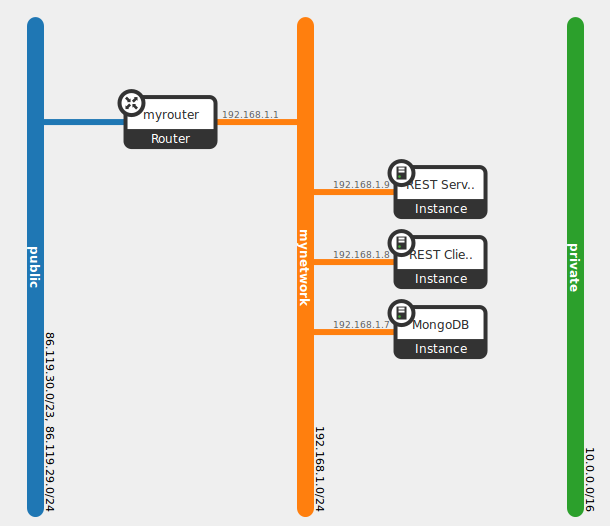
\includegraphics[width=80mm]{screen_network.png}
			\caption{Réseau privé créé}
		\end{figure}

		Un tel réseau permet de segmenter et séparer des groupes de machines qui n'ont pas lieu de communiquer entre elles. Cela apporte à la fois une organisation agréables des machines tout en fournissant un aspect sécuritaire, car si une machine était compromise, cela n'offrirait pas un accès à toutes les autres. De plus, il est ainsi possible de configurer des adresse \acs{IP} fixes dans ce réseau local, ce qui peut simplifier la mise en œuvre de l'application distribuée.

	\subtitledsection[Exercice 3]{Utiliser \openstackapi\ pour un déploiement automatique}

		Pour gérer automatiquement les instances, un script \brand{Bash} a été créé. Ce script à deux dépendances. La première est le fichier téléchargé par l'interface de \switchengines\ et nommé \code{openstack-rc-file.sh}. La seconde dépendance est une librairie de fonction d'aide à l'utilisation de l'\acs{API} \brand{Nova}. Ces fonctions ont étés créées pour cet exercice, afin de simplifier et rendre plus lisible le script final.

		Le script principal, nommé \code{run\_instances.sh} commence par démarrer les trois instances via la commande \code{nova boot} sur le réseau privé créé à l'exercice deux. Au lieu de démarrer des images, le script démarre des volumes \eng{bootable}. Ceci est pratique, car s'il l'on instancie un serveur depuis une image, cela créée à chaque fois un nouveau volume, qui ne sera pas automatiquement détruit. De plus, dans le cas du serveur de données (\mongodb) nous souhaiterions que les données accumulées soit conservées entre deux instanciations du serveur.

		Une fois les serveur instanciés, on attend qu'il soient "actifs", en vérifiant l'état retourné par la commande \code{nova list}. Dès que le serveur \mongodb\ est actif, on en récupère son adresse \acs{IP} locale qui servira à démarrer les autres serveurs. Il faut ensuite associer une adresse \acs{IP} flottante au serveur à démarrer et attendre qu'il soit possible de s'y connecter via un \acs{SSH}. Pour tester s'il est possible de se connecter via un \acs{SSH}, le plus simple (et peut-être même le plus pertinent) est de vérifier le résultat de la commande : \code{ssh -q <user>@<host> exit}. Le seul désavantage de cette manière de faire, est de devoir fournir des \eng{credentials} pour la connexion \acs{SSH}, là où la commande \code{nc} ne l'aurait pas nécessité. Mais comme de toute façon le script va avoir besoin d'utiliser ces \eng{credentials}, utiliser une manière alternative perd du sens. Avec une commande \acs{SSH}, on fait une vérification plus complète, en vérifiant non seulement la connexion réseau, mais aussi l'était du service, et de la possibilité d'authentification pour exécuter les commandes.

		Dès qu'il est possible de se connecter aux machines par \acs{SSH}, il suffit de démarrer les serveur via la commande \code{nohup} afin de ne pas bloquer le script de démarrage.

		Pour terminer, les instances sont simplement arrêtées et supprimées via la commande \code{nova delete}.

		\usemintedstyle{bw}
		\begin{minted}[
			frame=lines,
			fontsize=\footnotesize,
			linenos,
			label=Résultat de la commande : ./run\_instances.sh
		]{bash}
Instantiations ...
Wait for MongoDB ip ...
MongoDB ip is : 192.168.1.137
Start REST Client ...
Start REST Server ...
Services available at :
http://86.119.29.193:18000/getLastSensorsValues/pi1
http://86.119.29.193:18000/getLastSensorsValues/pi2
http://86.119.29.193:18000/getLastSensorsValues/pi3
Press 'A' (Abort) to stop instances :
Deleting instances ...
Instances deleted
		\end{minted}

	\section{Conclusion}
		Si pouvoir, créer et manipuler facilement des machines à la demande directement depuis une interface web est très pratique, on se rend très vite compte que pouvoir le faire par script, via une \acs{API} s'avère indispensable. En effet, l'interface, va surtout permettre de comprendre, et de faire quelques actions d'administration sur notre système. Mais dans la pratique, et plus particulièrement si l'on suit les principes de livraison continue des logiciels, ils est important de pouvoir déployer et gérer ses machines via des lignes de commandes.

		Si la \brand{Nova API} est très complète et permet d'effectuer toutes les actions nécessaire, il est tout de même dommage qu'il manque quelques utilitaires, typiquement pour simplement déterminer si un serveur donné est actif, ou pour obtenir l'adresse \acs{IP} d'un serveur, connaissant sont nom.

	\appendixsection

		\listoffigures

		\subsection{Acronymes utilisés}
			\begin{acronym}
				\defacronym{API}{Application Programming Interface}
				\defacronym{IP}{Internet Protocol}
				\defacronym{REST}{Representational State Transfert}
				\defacronym{SSH}{Secure Shell}
				\defacronym{URL}{Uniform Resource Location}
			\end{acronym}
			
		\subsection{Fichiers}
			Le présent rapport est livré avec les fichiers sources suivants :
			
			\begin{tabular}{l|l}
				nova-helper.sh & Utilitaires pour la manipulation de \brand{Nova API} développé dans le cadre de l'exercice \\ [1ex]
				run\_instances.sh & Script principal développé pour résoudre l'exercice 3 \\
			\end{tabular}
			
			\vspace{5mm}
			
			Les fichier \code{openstack-rc-file.sh} et \code{keypair.pem} qui sont nécessaires à l'exécution du script principal ne sont pas livrés. Ces fichiers ont simplement été téléchargés sur \switchengines\ sans être modifiés. Il contiennent donc uniquement des données personnelles de sécurité, sans aucun code écrit pour la résolution des exercices. De fait ces fichiers ne sont pas des sources pertinente pour accompagner ce rapport.
\end{document}
